\section{Pulse-Width Modulation (PWM)}

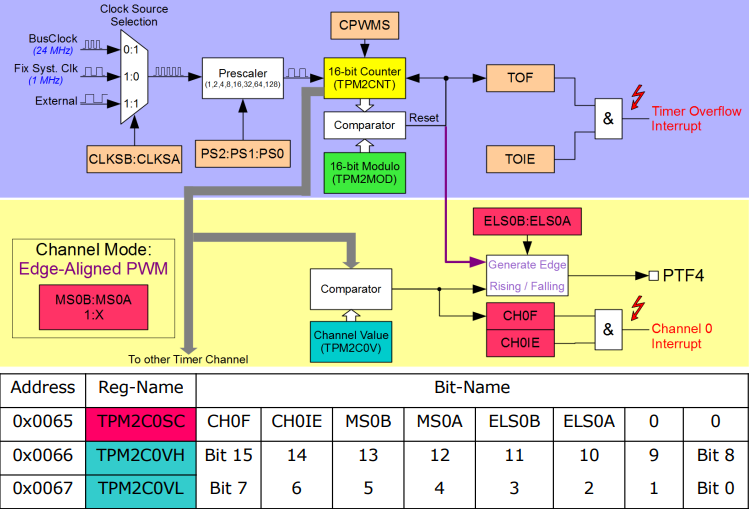
\includegraphics[width=0.5\textwidth]{edge-aligned-pwm-channel.png}

\subsection{Edge Aligned PWM}

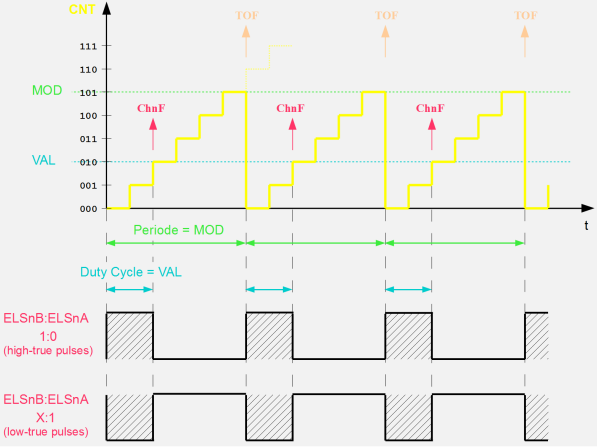
\includegraphics[width=0.5\textwidth]{signal-generation-edge-align-pwn.png}

\textit{
    VAL = 0: Duty Cycle = 0\% \newline
    VAL > MOD: Duty Cycle = 100\%
}

\begin{itemize}
    \item{
        \textit{
            \textbf{High-true pulses}: Das beduetet, dass true = 1 ist. Also solange der Channel Value >
            Counter ist, ist der ausgehende Pin = 1.
        }
    }
    \item{
        \textit{
            \textbf{Low-true pulses}: Das beduetet, dass true = 0 ist. Also solange der Channel Value >
            Counter ist, ist der ausgehende Pin = 0;
        }
    }
\end{itemize}

\subsection{H-Bridge (Fast / Slow Decay)}

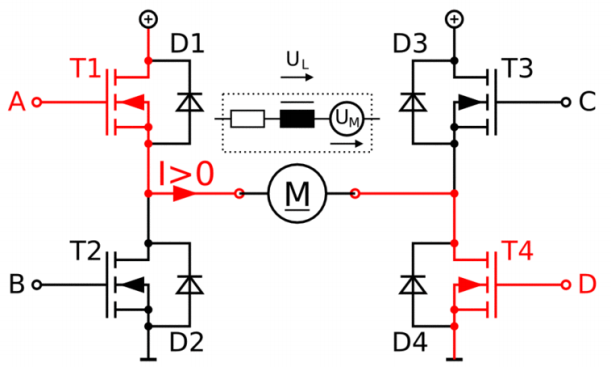
\includegraphics[width=0.5\textwidth]{h-bridge.png}

\textit{
    Energy in the Magnetic field
    \newline
    \textbf{Fast Decay}: "Brake"
    after T1 \& T4 on, deletion with D2
    \& D3 (2 x 0.7V Voltage drop $\rightarrow$ Power
    loss $\rightarrow$ eventually puls with T2 \& T3)
    \newline
    \textbf{Slow Decay}: "Idle Running"
    after T1 \& T4 on, delete with T2 \& T4
}

\subsection{PWM Code}

\begin{lstlisting}
void initTimer(void) {
    //set clock to 24 MHz
    TPM1SC_CLKSA = 1;
    TPM1SC_CLKSB = 0;
    //Prescaler to 0
    TPM1SC_PS0 = 0;
    TPM1SC_PS1 = 0;
    TPM1SC_PS2 = 0;
    // set Modulo to 2^16 -1 stellen.
    // (-1, to enable PWM to reach 100%)
    TPM1MOD = 65534;
}

void initPWM(void) {
    //Channel 2 to Mode Edge-Aligned PWM
    TPM1C2SC_MS2A = 1;
    TPM1C2SC_MS2B = 1;
    //set Channel 2 to "Low-true pulses", since LED rect to 0 as on
    TPM1C2SC_ELS2A = 1;
    TPM1C2SC_ELS2B = 1;
    //Channel 2 Channel Value = Modulo * 0.3, since set LED to 30%.
    TPM1C2V = 21844;
}

void main(void)
{
    // enable as output
    PTFDD_PTFDD0 = 1;

    initTimer();
    initPWM();

    for(;;);
}
\end{lstlisting}
